\begin{itemize}
    \item When moving processing to a high performance cluster there are two main gains:
        \begin{itemize}
            \item Parallelism, which greatly benefits this problem as it is 'embarrassingly parallel'
            \item Serial speed of each compute node (clusters are usually well specified w.r.t. RAM and CPU provisions)
        \end{itemize}
\end{itemize}

\subsection{Non-HEC}
Throughput for toolchain on a typical current system, say, an i5.  \todo{Run on my machine}


\subsection{HEC}
Times from the summary script\todo{median would be better; density plot of the below; plot vs. filesizes should be ~linear}.


\begin{figure}[h]
\centering
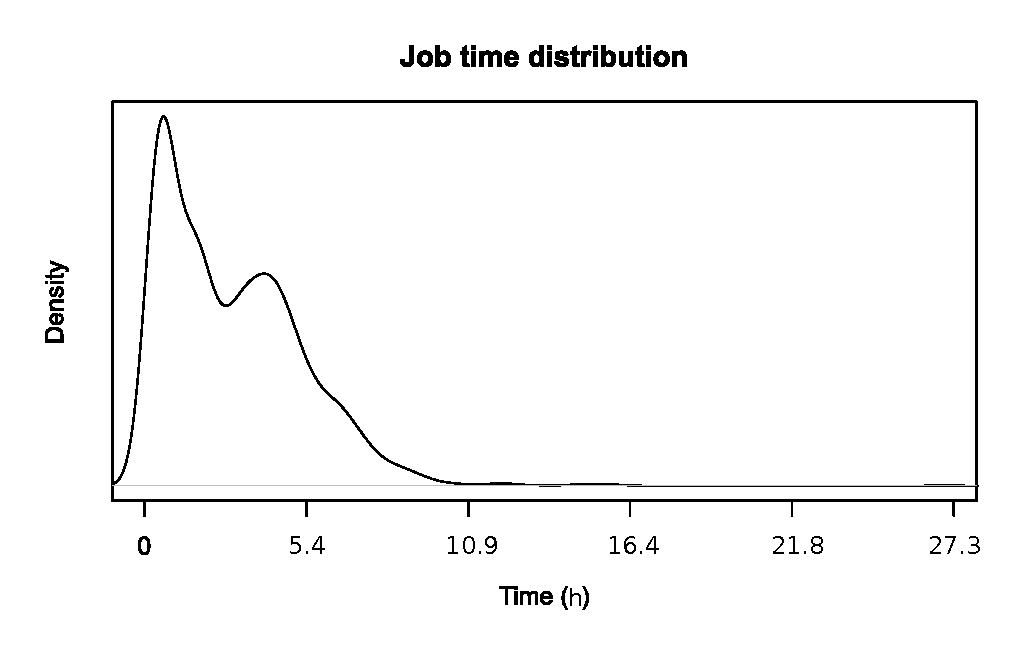
\includegraphics[width=0.5\textwidth]{jobtime.eps}
\caption{Distribution of job execution times on the HEC}
\label{fig:jobtimes}
\end{figure}



{\small
\begin{verbatim}
Total time (s): 24428748    ( / 60 / 60 / 24 = 282 days on the HPC )
Mean (s): 10955             ( / 60 / 60 = 3.04 hours )
Min (s): 223                ( / 60 = 3.7 minutes )
Max (s): 98872              ( / 60 / 60 = 27 hours )


> quantile(x$time, c(.05, .25, .50, .75, .95))
       5%       25%       50%       75%       95% 
 1248.897  3174.155  9321.105 16462.717 26126.913 
 20 mins   53 mins   2.5 hrs  4.5 hrs   7.25hrs
\end{verbatim}
}

Jobs were complete in 3 days.

"Each task runs all files in 20 directories through the tagger.  The other times are per-task could time info, just to give an idea of the variance.
The minimum is probably flawed because the list of directories was padded to be divisible by 20."

\begin{itemize}
    \item Throughput on HEC
    \item Scalability of HEC setup
\end{itemize}

